\documentclass[../documentation.tex]{subfiles}
 
\begin{document}
\section{Kameraválasztás, képkészítés programozása}
\subsection{Kameraválasztási szempontok, választott kamera}
A sakkbábuk pozíciójának felismerése képfeldolgozási eljáráson alapul. A képek készítéséhez használt kamera kiválasztásánál többféle szempont is szerepet játszott:
\begin{itemize}
	\item \underline{fekete-fehér/színes kép:} a zöld szín alapú bábukeresési eljáráshoz elengedhetetlen a színes képet szolgáltató kamera használata. QR-kód alapú felismeréshez megfelelő fekete-fehér kép is.
	\item \underline{felbontás:} ezt a legkisebb megkülönböztetni kívánt 2 fizikai pont távolsága, illetve a pontok kamerától vett távolsága egyaránt befolyásolja (később kerül részletes tárgyalásra).
	\item \underline{látószög:} ha a sakktábla kitölti a teljes képet, akkor a látószög azt határozza meg, hogy milyen távol lesz a kamera a tárgyaktól (a nem kifejezetten szűkített látóterű kamerák megfelelnek a célra).
	\item \underline{az illesztőszoftver (driver) kompatibilitása}: a projekthez valamilyen webkamera típus kiválasztása jó ötlet lehet a könnyű kezelhetőség, kedvező ár-érték arány és a viszonylag széles szoftveres támogatottság miatt. A robotvezérlőn Windows Embedded Standard 7 operációs rendszer fut, emiatt windows 7 kompatibilis webkamerát választottam.
\end{itemize} 

A sakktábla egy mezőjének mérete 40x40 mm, így az egész tábla 320x320 mm-es. A kalibráló kép ennél nagyobb, mivel az 10x9 cellából áll, ez így 400x360 mm. Egy sakkmezőt vízszintes és függőleges irányban is érdemes legalább 50 részre osztani (50x50=2500 pixelre), így a mezőkről készült kép megfelelően kivehető lesz. Ez azt jelenti, hogy 10*50, azaz 500 pixel szélesnek és magasnak kéne lennie a képnek legalább. Ezek alapján egy HD (1280*740 pixel) webkamerát választottam. 

\begin{figure}[h]
	\centering
	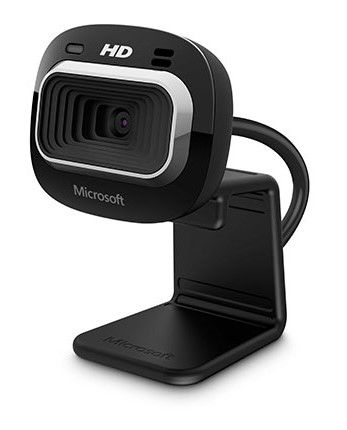
\includegraphics[height=60mm]{webcam-microsoft}
	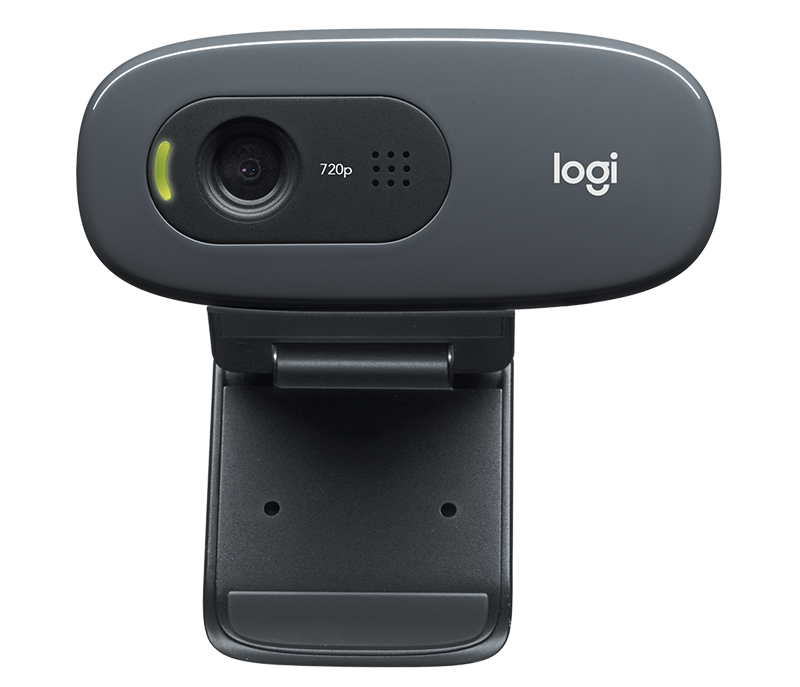
\includegraphics[height=55mm]{webcam-logitech}
	\caption{A projekthez kiindulásként használt Microsoft (balra) és a végső konstrukcióba beépített Logitech (jobbra) webkamera\protect\footnotemark}
	\label{fig:camera}
\end{figure}

Az első körben választott webkamera típusa: Microsoft LifeCam HD-3000. Az illesztőszoftver kizárólag Windows 7-re elérhető, de Windows 10 kompatibilis. Ennek ellenére a szoftver csak korlátozott funkciókkal működik Windows 7 alatt. Ezen kamera választásának másik hátránya, hogy az illesztőszoftver telepítője nem \angol{offline}. Ez azért lehet probléma, mert a robotvezérlő alapvetően nem rendelkezik internethozzáféréssel, emiatt a telepítés kifejezetten körülményes. \angol{Windows Embedded Standard} 7 (WES7) operációs rendszerrel nem sikerült kompatibilissá tenni az illesztőszoftvert.

A második választás a Logitech C270 HD webkamerára esett. Az illesztőszoftver alapvetően Windows 7-hez készült. Az illesztőprogram telepítője \angol{offline} működik. További előny, hogy az illesztőprogrammal együtt a gyártó saját alkalmazását is telepíti hozzá, amivel a kamera képét \angol{stream}-ként lehet nézni. Erre alkalmas lenne a Windows verziókban általában elérhető kamera alkamazás is, de ez WES7 esetén nem alapfunkció. A saját alkalmazással így a kamerát a robotvezérlőhöz kötve is elvégezhetjük a megfelelő kamerapozíció beállítását, nincs szükség külön laptopra.

\footnotetext{A Microsoft kamera képének linkje: https://www.microsoft.com/accessories/hu-hu/products/webcams/lifecam-hd-3000/t3h-00004\\
A Logitech kamerájé: https://www.logitech.com/hu-hu/product/hd-webcam-c270}


\subsection{Képkészítés OpenCV-vel}
A webkamerát a programon belül OpenCV-s függvények kezelik. A szükséges metódusokat az `imgprocess' csomagban található `CameraHandler.java' fájl tartalmazza. Az alábbi függvények kerültek implementálásra:
\begin{itemize}
	\item \underline{CameraHandler konstruktor:} az osztály példányosításakor paraméterként azt a számot kell megadni, ahanyadik indexű a kamera az elérhető képkészítő eszközök listájában (a robotvezérlőhöz ha nincs más kamera csatlakoztatva, akkor ez a 0. index). Sajnálatos módon OpenCV-ben nem lehet kilistázni az elérhető kamerákat, és például név alapján kikeresni a megfelelő kamerát. A konstruktor a képkészítés felbontását HD-ra állítja (ha ez nincs definiálva, akkor a program nem feltétlen ezt választja).
	\item \underline{grabFrame:} ez a metódus adja vissza a csatlakoztatott kamera által készített képeket (BufferedImage).
	\item \underline{rotateClockwise90:} erre a függvényre azért van szükség, mert a kamera a robotkarra 90°-kal elforgatva lett felszerelve az képfeldolgozó eljárások által várt orientációhoz képest.
	\item \underline{closeCamera:} ha már a kamera nincs használatban, ezzel a függvénnyel lehet inaktívvá tenni.
\end{itemize}

\begin{figure}[h]
	\centering
	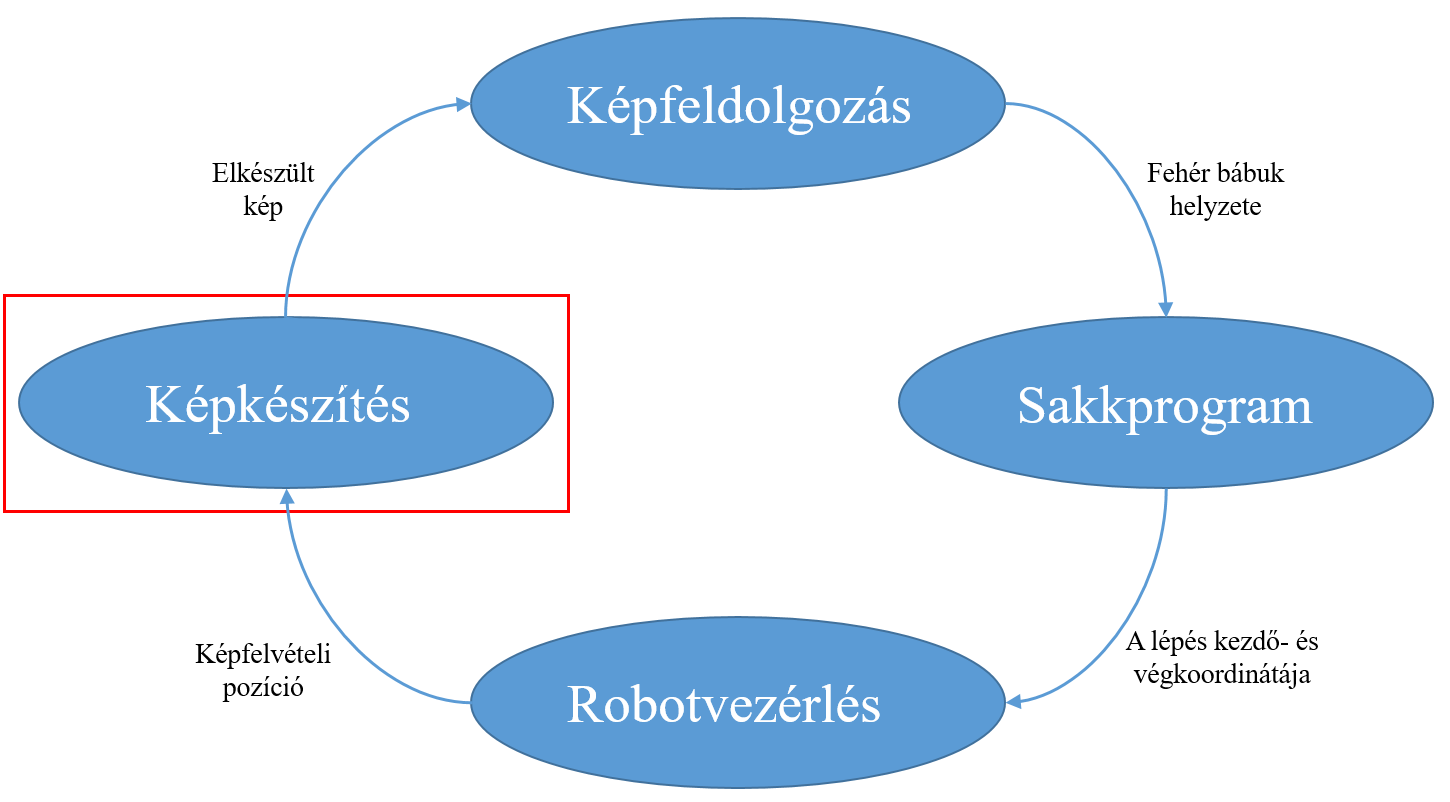
\includegraphics[scale=0.35]{flowchart-takeimage}
	\caption{Képkészítés helye a folyamatban}
	\label{fig:camera}
\end{figure}





























\end{document}